\section{Introduction}
\begin{figure}[t]
\begin{center}
   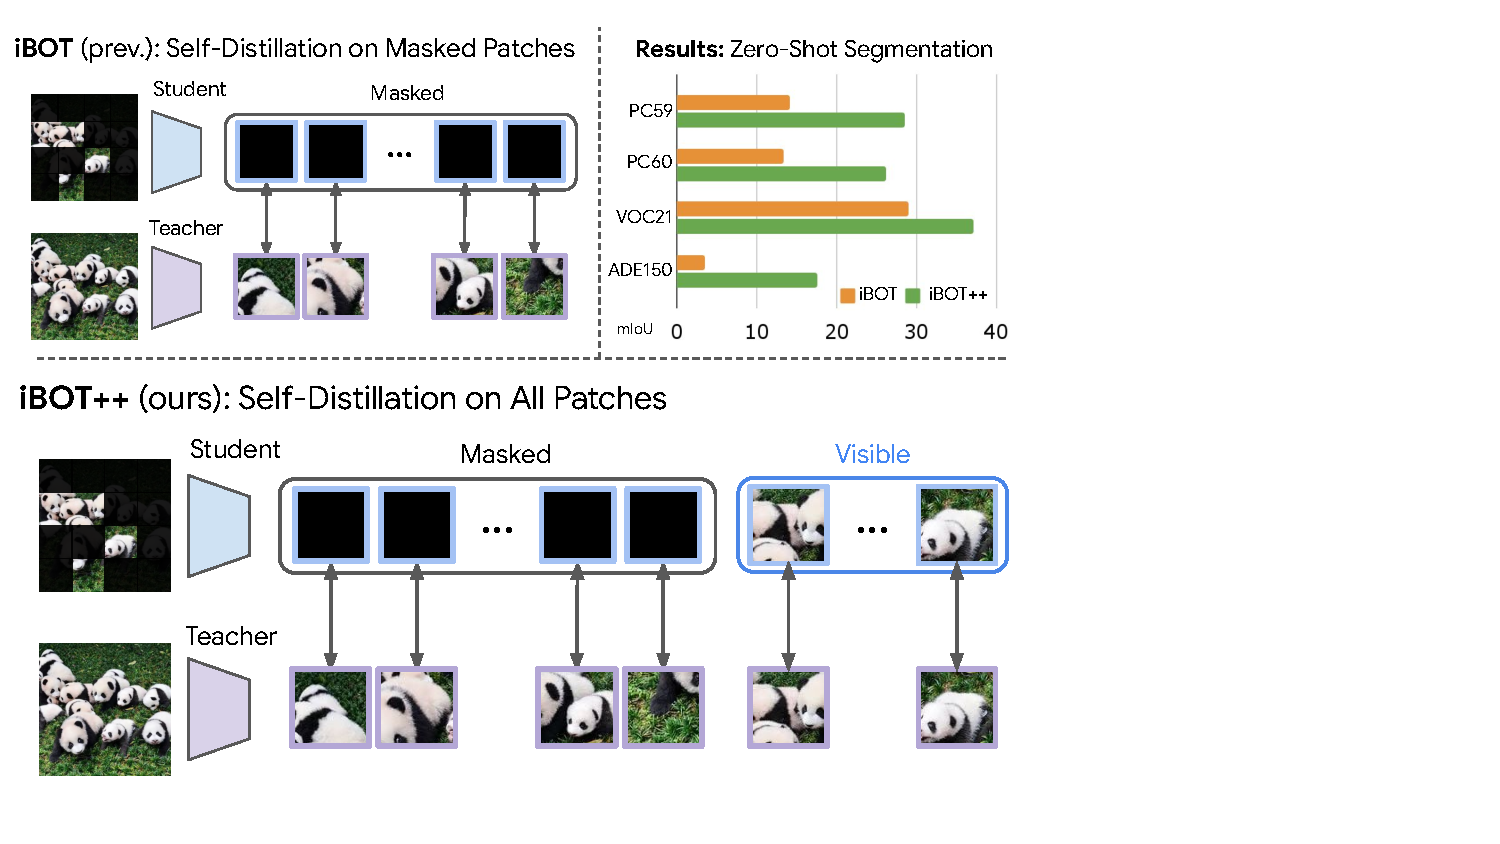
\includegraphics[width=1.0\linewidth]{figures/tipsv2_teaser_compact.pdf}
\end{center}
\vspace{-0.1in}
  \caption{
  \textbf{\tipsvtwo's improvement to the masked image modeling pretraining strategy.}
  As part of our complete \tipsvtwo method, we introduce iBOT++ (bottom), a simple modification to the well-known iBOT~\cite{zhou2022ibot} self-supervised objective (top-left), where visible tokens also contribute directly to the loss.
  This enhancement dramatically improves patch-text alignment, as demonstrated by zero-shot image segmentation results (top-right).
 }
\label{fig:teaser_compact}
\end{figure}

    


Large-scale self-supervised and vision-language pretraining methods have fundamentally reshaped visual representation learning, establishing new performance standards across a broad spectrum of tasks. 
Leading approaches generally fall into two categories: weakly-supervised contrastive or sigmoid methods, exemplified by CLIP~\citep{radford2021clip}, SigLIP ~\citep{zhai2023siglip} and Perception Encoder (PE)~\citep{bolya2025perceptionencoderbestvisual}, which provide robust image-text alignment and zero-shot capabilities; and self-supervised learning (SSL) methods, such as DINO~\citep{siméoni2025dinov3,caron2021dino,oquab2024dinov2} and iBOT~\citep{zhou2022ibot}, which excel at spatial understanding for dense downstream tasks (e.g., depth, segmentation).

Achieving a unified representation that excels simultaneously at global (image-level) and dense (patch-level) understanding remains a significant challenge. State-of-the-art (SOTA) models often optimize one at the expense of the other: for example, DINOv2~\citep{oquab2024dinov2} excels at dense vision tasks but lacks inherent text alignment for vision-language capabilities, whereas PE-core~\citep{bolya2025perceptionencoderbestvisual} provides robust image-text alignment but underperforms on dense tasks. 
Recent unified approaches, such as TIPS~\citep{tips_paper} and SigLIP2~\citep{tschannen2025siglip2multilingualvisionlanguage}, have made significant strides in bridging this divide. 
However, we find that even these modern models struggle to maintain precise pixel- or patch-level alignment with text—a capability essential for advanced tasks like open-vocabulary segmentation. 
Self-supervised works such as DINO.txt~\citep{jose2024dinov2} and DINOv3~\citep{siméoni2025dinov3} attempt to address this by training supplementary text encoders, but still exhibit limited performance on multimodal tasks. 
Overall, grounded alignment with text remains a challenging task. 
This is corroborated by PE~\citep{bolya2025perceptionencoderbestvisual}, which finds that final transformer layers often function as global contrastive ``decoders'', rather than preserving the local semantics.

In this work, we first uncover a surprising trend in SOTA vision encoders ~\citep{tips_paper, tschannen2025siglip2multilingualvisionlanguage}: the largest flagship models often underperform their smaller counterparts in patch-text alignment. 
Investigating this issue with a recent spatially-aware multimodal encoder~\citep{tips_paper}, we find that distillation significantly improves grounding alignment by applying effective supervision across all patch tokens. 
This insight not only explains the performance gap, but also helps us unlock broader capabilities through a novel pretraining recipe. 

We introduce \textbf{\tipsvtwo}, the second version of the TIPS~\cite{tips_paper} model family (\textbf{T}ext-\textbf{I}mage \textbf{P}retraining with \textbf{S}patial awareness), a novel methodology designed to bridge this gap directly during pretraining.
\tipsvtwo incorporates a new objective, iBOT++, which translates our distillation findings into a self-supervised pretraining objective that enforces representation consistency on visible tokens, as per \cref{fig:teaser_compact}. 
We further enhance this with multi-granularity text augmentation (leveraging captions from PaliGemma ~\citep{beyer2024paligemma} and Gemini ~\citep{geminiteam2024gemini}) and a resource-efficient Exponential Moving Average (EMA) strategy. 
While standard SSL often requires full-model EMA, the presence of text supervision allows us to use a `head-only EMA'.
This updates only the projection layers, drastically reducing memory requirements at training time.
\tipsvtwo provides an efficient training framework yielding a highly effective image-text encoder across standard benchmarks. 
It sets new SOTA results in zero-shot semantic segmentation, while providing strong performance on a wide range of downstream multimodal tasks.
In summary, our primary contributions are:
\begin{itemize}
\item A novel finding that a distillation procedure tuned to strengthen spatial awareness unlocks strong gains in patch-text alignment.
Our detailed study pinpoints masking removal and initialization as the key factors driving this phenomenon.
\item iBOT++, a novel self-supervised masked objective that enhances pretraining to enforce representation consistency and significantly improves patch-text alignment -- see \cref{fig:teaser_compact}.
\item An efficient and effective training recipe leveraging multi-granularity text augmentation and a novel head-only EMA mechanism, overall achieving strong performance with significantly reduced training cost, validated comprehensively on 9 tasks spanning 20 datasets. 

\end{itemize}

